\documentclass[border=10pt, multi, tikz]{standalone}
\usepackage{import}
\subimport{../settings/}{init}
\usetikzlibrary{positioning}
\usetikzlibrary{calc}

% Colors -----------------------------------------------------------------------

% Background and boxes											% --HEX--
\definecolor{background}{HTML}{1A1B26}			% #1A1B26
\definecolor{boxcolor}{HTML}{24283B}				% #24283B
\definecolor{commentscolor}{HTML}{565F89}		% #565F89
\definecolor{darkred}{HTML}{D72323}					% #D72323
\definecolor{darkblue}{HTML}{0A84FF}				% #0A84FF
\definecolor{darkgreen}{HTML}{00C853}				% #00C853
\definecolor{darkyellow}{HTML}{FFCB30}			% #FFCB30

% Text shades																% --HEX--				
\definecolor{black}{HTML}{000000}						% #000000
\definecolor{darkgray}{HTML}{161B22}				% #161B22
\definecolor{gray}{HTML}{89929B}						% #89929B
\definecolor{lightgray}{HTML}{C6CDD5}				% #C6CDD5
\definecolor{white}{HTML}{FFFFFF}						% #FFFFFF
\definecolor{textcolor}{HTML}{FFFFFF}       % #FFFFFF

% Colors                                    % --HEX--
\definecolor{red}{HTML}{F7768E}             % #F7768E
\definecolor{orange}{HTML}{FF9E64}          % #FF9E64
\definecolor{yellow}{HTML}{FFCB30}          % #FFCB30
\definecolor{green}{HTML}{9ECE6A}           % #9ECE6A
\definecolor{azure}{HTML}{2AC3DE}           % #2AC3DE
\definecolor{blue}{HTML}{7AA2F7}            % #7AA2F7
\definecolor{purple}{HTML}{BB9AF7}          % #BB9AF7

% Background and text color
\pagecolor{background}                      % Page Background
\color{textcolor}                           % Main text color
\colorlet{captionscolor}{gray}							% Caption Colors
\colorlet{iconscolor}{white}								% Icons color
\colorlet{linescolor}{gray}									% Lines color
\colorlet{numerscolor}{commentscolor}				% Line Numbers color

% Other colors
\definecolor{rrr}{HTML}{FF0000}
\definecolor{ggg}{HTML}{00FF00}
\definecolor{bbb}{HTML}{0000FF}


% White background
% \def\ConvColor{rgb:yellow,5;red,2.5;white,5}
% \def\ConvReluColor{rgb:yellow,5;red,5;white,5}
% \def\PoolColor{rgb:red,1;black,0.3}
% \def\UnpoolColor{rgb:blue,2;green,1;black,0.3}
% \def\ConcatColor{rgb:blue,5;red,2.5;white,5}
% \def\FcReluColor{rgb:blue,5;red,5;white,4}
% \def\SoftmaxColor{rgb:magenta,5;black,7}

% Dark Background
\def\ConvColor{commentscolor}
\def\ConvReluColor{commentscolor}
% \def\ConvReluColor{yellow!50!commentscolor}
\def\PoolColor{red}
\def\UnpoolColor{azure}
% \def\UnpoolColor{azure!30!purple}
\def\ConcatColor{purple}
\def\BatchColor{background}
% \def\BatchColor{yellow}

% for the presentation images
% \def\ConvColor{background}
% \def\ConvColor{yellow}
% \def\ConvReluColor{background}
% \def\ConvReluColor{yellow}
% \def\PoolColor{background}
% \def\UnpoolColor{background}
% \def\ConcatColor{background}
% \def\BatchColor{background}


% Other Commands ---------------------------------------------------------------

\newcommand{\normmidarrow}{
	\tikz \draw[-Stealth,
							line width =0.8mm,
							draw=gray,
						] (-0.3,0) -- ++(0.3,0);
}

\newcommand{\copymidarrow}{
	\tikz \draw[-Stealth,
							line width =0.8mm,
							draw=\ConcatColor,
							% draw={rgb:blue,4;red,1;green,1;black,3}
						] (-0.3,0) -- ++(0.3,0);
}

\begin{document}
\begin{tikzpicture}

\tikzstyle{connection}=[
	ultra thick,
	every node/.style={sloped,allow upside down},
	draw=\edgecolor,
	opacity=0.7
]

\tikzstyle{poolconnection}=[
	ultra thick,
	every node/.style={sloped,allow upside down},
	draw=\PoolColor,
	opacity=0.7
]

\tikzstyle{unpoolconnection}=[
	ultra thick,
	every node/.style={sloped,allow upside down},
	draw=\UnpoolColor,
	opacity=0.7
]

\tikzstyle{normconnection}=[
	ultra thick,
	every node/.style={sloped,allow upside down},
	draw=gray,
	opacity=0.7
]

\tikzstyle{copyconnection}=[
	ultra thick,
	every node/.style={sloped,allow upside down},
	draw=\ConcatColor,
	% draw={rgb:blue,4;red,1;green,1;black,3},
	opacity=0.7
]


% Encoder ----------------------------------------------------------------------

% Convolution 11 and 12
\pic[shift={(0,0,0)}] at (0,0,0) {
	RightBandedBox={
		name=cr1,
		xlabel={{"32","32"}},
		caption=Encoder 1,
		fill=\ConvColor,
		bandfill=\ConvReluColor,
		height=40,
		width={2,2},
		depth=40
	}
};
\node[rotate=45] at ($(cr1-south) + (0.8,0)$) {$240 \times 240$};
\node[rotate=45] at ($(cr1-north) + (0,0,-6)$) {
	\shortstack{$7 \times 7$ conv \\ ReLU \\ \textcolor{\BatchColor}{BN}}
};

% Pooling 1
\pic[shift={(1.2,-10,0)}] at (cr1-east) {
	Box={
		name=p1,
		xlabel={{"32",""}},
		fill=\PoolColor,
		opacity=0.6,
		height=32,
		width=2,
		depth=32
	}
};
\node[rotate=45] at ($(p1-north) + (0,0,-6.2)$) {\textcolor{\PoolColor}{$2 \times 2$
max pool}};

% Convolution 21 and 22
\pic[shift={(0,0,0)}] at (p1-east) {
	RightBandedBox={
		name=cr2,
		xlabel={{"64","64"}},
		caption=Encoder 2,
		fill=\ConvColor,
		bandfill=\ConvReluColor,
		height=32,
		width={3.5,3.5},
		depth=32
	}
};
\node[rotate=45] at ($(cr2-south) + (1.1,0)$) {$120 \times 120$};
\node[rotate=45] at ($(cr2-north) + (0,0,-5.3)$) {
	\shortstack{$7 \times 7$ conv \\ ReLU \\ \textcolor{\BatchColor}{BN}}
};

% Pooling 2
\pic[shift={(1.2,-8.5,0)}] at (cr2-east) {
	Box={
		name=p2,
		xlabel={{"64",""}},
		fill=\PoolColor,
		opacity=0.6,
		height=25,
		width=3,
		depth=25
	}
};
\node[rotate=45] at ($(p2-north) + (0,0,-5.5)$) {\textcolor{\PoolColor}{$2 \times 2$
max pool}};

% Convolution 31 and 32
\pic[shift={(0,0,0)}] at (p2-east) {
	RightBandedBox={
		name=cr3,
		xlabel={{"128","128"}},
		caption=Encoder 3,
		fill=\ConvColor,
		bandfill=\ConvReluColor,
		height=25,
		width={4.5,4.5},
		depth=25
	}
};
\node[rotate=45] at ($(cr3-south) + (1.3,0)$) {$60 \times 60$};
\node[rotate=45] at ($(cr3-north) + (0,0,-4.6)$) {
	\shortstack{$7 \times 7$ conv \\ ReLU \\ \textcolor{\BatchColor}{BN}}
};

% Pooling 3
\pic[shift={(1.2,-6.5,0)}] at (cr3-east) {
	Box={
		name=p3,
		xlabel={{"128",""}},
		fill=\PoolColor,
		opacity=0.6,
		height=16,
		width=4.5,
		depth=16
	}
};
\node[rotate=45] at ($(p3-north) + (0,0,-4.5)$) {\textcolor{\PoolColor}{$2 \times 2$
max pool}};

% Convolution 41, 42, and 43
\pic[shift={(0,0,0)}] at (p3-east) {
	RightBandedBox={
		name=cr4,
		xlabel={{"256","256"}},
		caption=Encoder 4,
		fill=\ConvColor,
		bandfill=\ConvReluColor,
		height=16,
		width={6,6},
		depth=16
	}
};
\node[rotate=45] at ($(cr4-south) + (1.6,0)$) {$30 \times 30$};
\node[rotate=45] at ($(cr4-north) + (0,0,-3.8)$) {
	\shortstack{$7 \times 7$ conv \\ ReLU \\ \textcolor{\BatchColor}{BN}}
};

% Pooling 4
\pic[shift={(1.2,-5,-0.5)}] at (cr4-east) {
	Box={
		name=p4,
		xlabel={{"256",""}},
		fill=\PoolColor,
		opacity=0.6,
		height=8,
		width=6,
		depth=8
	}
};
\node[rotate=45] at ($(p4-north) + (0,0,-3.8)$) {\textcolor{\PoolColor}{$2 \times 2$
max pool}};	


% Bottleneck -------------------------------------------------------------------

% Convolution 51, 52, and 53
\pic[shift={(0,0,0)}] at (p4-east) {
	RightBandedBox={
		name=cr5,
		xlabel={{"256$\rightarrow$1024$\rightarrow$","256$\rightarrow$1024$\rightarrow$256"}},
		caption=Bottleneck,
		fill=\ConvColor,
		bandfill=\ConvReluColor,
		height=8,
		width={12,12},
		depth=8
	}
};
\node[rotate=45] at ($(cr5-south) + (2.8,0)$) {$15 \times 15$};
\node[rotate=45] at ($(cr5-north) + (0,0,-3)$) {
	\shortstack{$7 \times 7$ conv \\ ReLU \\ \textcolor{\BatchColor}{BN}}
};


% Decoder ----------------------------------------------------------------------

%  Unpooling 4
% \pic[shift={(1.5,3,0)}] at (cr5-north) {
\pic[shift={(3,5,0.5)}] at (cr5-east) {
	Box={
		name=up4,
		xlabel={{"256",""}},
		fill=\UnpoolColor,
		opacity=0.6,
		height=16,
		width=6,
		depth=16
	}
};
\node[rotate=45] at ($(up4-north) + (-0.4,0,-4.3)$) {
	\textcolor{\UnpoolColor}{\shortstack{$2\times$ Bilinear \\ Upsampling}}
};

% Residual Connection 4
\pic[shift={(-1.2,0,0)}] at (up4-west) {
% \pic[shift={(0,0,0)}] at (up4-west) {
	Box={
		name=cat4,
		xlabel={{"256",""}},
		fill=\ConcatColor,
		height=16,
		width=6,
		depth=16
	}
};
\node[rotate=45] at ($(cat4-north) + (-1.6,0,-4.5)$) {
	\textcolor{\ConcatColor}{\shortstack{Residual \\ Connection}}
};

% Convolution 41, 42, and 43
\pic[shift={(0,0,0)}] at (up4-east) {
	RightBandedBox={
		name=ucr4,
		xlabel={{"256","256"}},
		caption=Decoder 4,
		fill=\ConvColor,
		bandfill=\ConvReluColor,
		height=16,
		width={6,6},
		depth=16
	}
};
\node[rotate=45] at ($(ucr4-south) + (1.6,0)$) {$30 \times 30$};
\node[rotate=45] at ($(ucr4-north) + (0,0,-3.8)$) {
	\shortstack{$7 \times 7$ conv \\ ReLU \\ \textcolor{\BatchColor}{BN}}
};

% Unpooling 3
\pic[shift={(3.5,6.5,0)}] at (ucr4-east) {
	Box={
		name=up3,
		xlabel={{"128",""}},
		fill=\UnpoolColor,
		opacity=0.6,
		height=25,
		width=4.5,
		depth=25
	}
};
\node[rotate=45] at ($(up3-north) + (-0.3,0,-5.2)$) {
	\textcolor{\UnpoolColor}{\shortstack{$2\times$ Bilinear \\ Upsampling}}
};

% Residual Connection 3
\pic[shift={(-0.9,0,0)}] at (up3-west) {
% \pic[shift={(0,0,0)}] at (up3-west) {
	Box={
		name=cat3,
		xlabel={{"128",""}},
		fill=\ConcatColor,
		height=25,
		width=4.5,
		depth=25
	}
};
\node[rotate=45] at ($(cat3-north) + (-1.4,0,-5.6)$) {
	\textcolor{\ConcatColor}{\shortstack{Residual \\ Connection}}
};

% Convolution 31 and 32
\pic[shift={(0,0,0)}] at (up3-east) {
	RightBandedBox={
		name=ucr3,
		xlabel={{"128","128"}},
		caption=Decoder 3,
		fill=\ConvColor,
		bandfill=\ConvReluColor,
		height=25,
		width={4.5,4.5},
		depth=25
	}
};
\node[rotate=45] at ($(ucr3-south) + (1.3,0)$) {$60 \times 60$};
\node[rotate=45] at ($(ucr3-north) + (0,0,-4.6)$) {
	\shortstack{$7 \times 7$ conv \\ ReLU \\ \textcolor{\BatchColor}{BN}}
};

% Unpooling 2
\pic[shift={(3.8,8.5,0)}] at (ucr3-east) {
	Box={
		name=up2,
		xlabel={{"64",""}},
		fill=\UnpoolColor,
		opacity=0.6,
		height=32,
		width=3.5,
		depth=32
	}
};
\node[rotate=45] at ($(up2-north) + (-0.3,0,-5.8)$) {
	\textcolor{\UnpoolColor}{\shortstack{$2\times$ Bilinear \\ Upsampling}}
};

% Residual Connection 2
\pic[shift={(-0.7,0,0)}] at (up2-west) {
% \pic[shift={(0,0,0)}] at (up2-west) {
	Box={
		name=cat2,
		xlabel={{"64",""}},
		fill=\ConcatColor,
		height=32,
		width=3.5,
		depth=32
	}
};
\node[rotate=45] at ($(cat2-north) + (-1.4,0,-6.2)$) {
	\textcolor{\ConcatColor}{\shortstack{Residual \\ Connection}}
};

% Convolution 21 and 22
\pic[shift={(0,0,0)}] at (up2-east) {
	RightBandedBox={
		name=ucr2,
		xlabel={{"64","64"}},
		caption=Decoder 2,
		fill=\ConvColor,
		bandfill=\ConvReluColor,
		height=32,
		width={3.5,3.5},
		depth=32
	}
};
\node[rotate=45] at ($(ucr2-south) + (1.1,0)$) {$120 \times 120$};
\node[rotate=45] at ($(ucr2-north) + (0,0,-5.3)$) {
	\shortstack{$7 \times 7$ conv \\ ReLU \\ \textcolor{\BatchColor}{BN}}
};

% Unpooling 1
\pic[shift={(5,10,0)}] at (ucr2-east) {
	Box={
		name=up1,
		xlabel={{"32",""}},
		fill=\UnpoolColor,
		opacity=0.6,
		height=40,
		width=2,
		depth=40
	}
};
\node[rotate=45] at ($(up1-north) + (-0.4,0,-6.8)$) {
	\textcolor{\UnpoolColor}{\shortstack{$2\times$ Bilinear \\ Upsampling}}
};

% Residual Connection 1
\pic[shift={(-0.4,0,0)}] at (up1-west) {
% \pic[shift={(0,0,0)}] at (up1-west) {
	Box={
		name=cat1,
		xlabel={{"32",""}},
		fill=\ConcatColor,
		height=40,
		width=2,
		depth=40
	}
};
\node[rotate=45] at ($(cat1-north) + (-1.5,0,-7.3)$) {
	\textcolor{\ConcatColor}{\shortstack{Residual \\ Connection}}
};

% Convolution 11 and 12
\pic[shift={(0,0,0)}] at (up1-east) {
	RightBandedBox={
		name=ucr1,
		xlabel={{"32","32"}},
		caption=Decoder 1,
		fill=\ConvColor,
		bandfill=\ConvReluColor,
		height=40,
		width={2,2},
		depth=40
	}
};
\node[rotate=45] at ($(ucr1-south) + (0.8,0)$) {$240 \times 240$};
\node[rotate=45] at ($(ucr1-north) + (0.4,0,-6)$) {
	\shortstack{$7 \times 7$ conv \\ ReLU \\ \textcolor{\BatchColor}{BN}}
};


% Output image -----------------------------------------------------------------
\pic[shift={(3.5,0,0)}] at (ucr1-east) {
	Box={
		name=outred,
		fill=rrr,
		height=40,
		width=1.5,
		depth=40
	}
};
\pic[shift={(0,0,0)}] at (outred-east) {
	Box={
		name=outgreen,
	caption=\mbox{Output} \mbox{image},
		fill=ggg,
		height=40,
		width=1.5,
		depth=40
	}
};
\pic[shift={(0,0,0)}] at (outgreen-east) {
	Box={
		name=outblue,
		fill=bbb,
		height=40,
		width=1.5,
		depth=40
	}
};
\node[rotate=45] at ($(outblue-south) + (0.5,0)$) {$240 \times 240$};


% Input image -----------------------------------------------------------------
\pic[shift={(-5.5,0,0)}] at (cr1-east) {
	Box={
		name=input1,
		fill=gray,
		height=40,
		width=1.5,
		depth=40
	}
};
\pic[shift={(0,0,0)}] at (input1-east) {
	Box={
		name=input2,
		fill=gray,
		caption=\mbox{Input} \mbox{Scans},
		height=40,
		width=1.5,
		depth=40
	}
};
\pic[shift={(0,0,0)}] at (input2-east) {
	Box={
		name=input3,
		fill=gray,
		height=40,
		width=1.5,
		depth=40
	}
};
\pic[shift={(0,0,0)}] at (input3-east) {
	Box={
		name=input4,
		fill=gray,
		height=40,
		width=1.5,
		depth=40
	}
};
\node[rotate=45] at ($(input4-south) + (0.5,0)$) {$240 \times 240$};


% Draw connections ------------------------------------------------------------

% Residual / Skip connections
\draw[copyconnection]  (cr4-east)  -- node {\copymidarrow} (cat4-west);
\draw[copyconnection]  (cr3-east)  -- node {\copymidarrow} (cat3-west);
\draw[copyconnection]  (cr2-east)  -- node {\copymidarrow} (cat2-west);
\draw[copyconnection]  (cr1-east)  -- node {\copymidarrow} (cat1-west);

% Pooling connection 1
\path (cr1-east) -- (p1-north|-cr1-west) coordinate[pos=1] (crp1-mid);
\draw[poolconnection] (cr1-east) -- (crp1-mid);
\draw[poolconnection,-Stealth] (p1-north|-crp1-mid) -- (p1-north);

% Pooling connection 2
\path (cr2-east) -- (p2-north|-cr2-west) coordinate[pos=1] (crp2-mid);
\draw[poolconnection] (cr2-east) -- (crp2-mid);
\draw[poolconnection,-Stealth] (p2-north|-crp2-mid) -- (p2-north);

% Pooling connection 3
\path (cr3-east) -- (p3-north|-cr3-west) coordinate[pos=1] (crp3-mid);
\draw[poolconnection] (cr3-east) -- (crp3-mid);
\draw[poolconnection,-Stealth] (p3-north|-crp3-mid) -- (p3-north);

% Pooling connection 4
\path (cr4-east) -- (p4-north|-cr4-west) coordinate[pos=1] (crp4-mid);
\draw[poolconnection] (cr4-east) -- (crp4-mid);
\draw[poolconnection,-Stealth] (p4-north|-crp4-mid) -- (p4-north);

% Unpooling connection 4
\path (cr5-east) -- (up4-south|-cr5-east) coordinate[pos=0.81] (crup4-mid);
\draw[unpoolconnection,-Stealth] (cr5-east) -- (crup4-mid) -- ($(crup4-mid) +
(0, 2.1)$);
% \draw[unpoolconnection,-Stealth] (up4-south|-crup4-mid) -- (up4-south);
% \draw[unpoolconnection,-Stealth] (up4-south|-crup4-mid) -- ($(up4-south) + (0, -1)$);

% Unpooling connection 3
\path (ucr4-east) -- (up3-south|-ucr4-east) coordinate[pos=0.75] (ucrup3-mid);
\draw[unpoolconnection,-Stealth] (ucr4-east) -- (ucrup3-mid) -- ($(ucrup3-mid) +
(0, 2.6)$);

% Unpooling connection 2
\path (ucr3-east) -- (up2-south|-ucr3-east) coordinate[pos=0.69] (ucrup2-mid);
\draw[unpoolconnection,-Stealth] (ucr3-east) -- (ucrup2-mid) -- ($(ucrup2-mid) +
(0, 3.6)$);

% Unpooling connection 1
\path (ucr2-east) -- (up1-south|-ucr2-east) coordinate[pos=0.72] (ucrup1-mid);
\draw[unpoolconnection,-Stealth] (ucr2-east) -- (ucrup1-mid) -- ($(ucrup1-mid) +
(0, 3.3)$);

% Output Image connection
\draw[normconnection]  (ucr1-east)  -- node {\normmidarrow} (outred-west);

% Input Image connection
\draw[normconnection]  (input4-east)  -- node {\normmidarrow} (cr1-west);


% Separable Convolutions ------------------------------------------------------

% Small zoom-in circle
\draw[draw=textcolor,
			fill=gray!50!background,
			opacity=0.75, 
			line width=1.5
		] (-1,0) circle (1.5);

% Cone borders
\draw[draw=textcolor, 
			opacity=1, 
			line width=1.5,
			] (0.5, -0.5) -- (10, -5);

% Big zoom-in circle
\draw[draw=textcolor, 
			fill=background, 
			opacity=1, 
			line width=1
		] (27,-12.5) circle (19);

% % Normal Convolution Image
% \node at (27,-15) {
% 	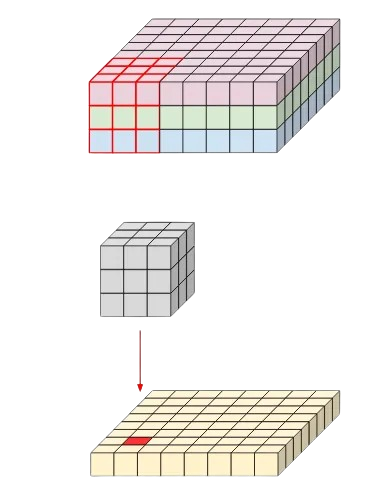
\includegraphics[width=1.8\textwidth, angle=90]{normal-convolution2.png}
% };
% \node at (27,-4) {
% 	\fontsize{30}{30}\selectfont \textcolor{textcolor}{\textbf{Normal Convolution}}
% };

% Separable Convolution Image
\node at (27,-15) {
	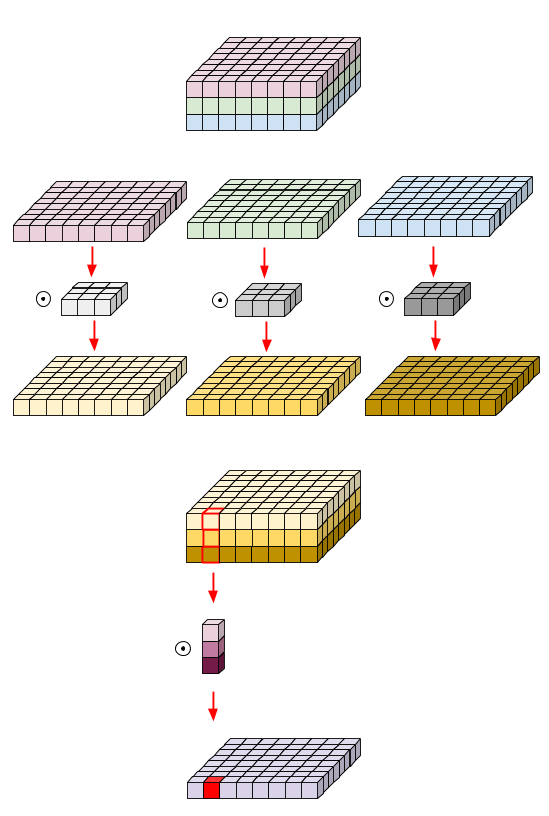
\includegraphics[width=1.8\textwidth, angle=90]{separable-convolution.png}
};
\node at (27,-2) {
	\fontsize{30}{30}\selectfont \textcolor{textcolor}{\textbf{Separable Convolution}}
};


\end{tikzpicture}
\end{document}
